\documentclass[png={size=500x500},border=100pt]{standalone}

\usepackage{tikz}
\usetikzlibrary{calc}

\definecolor{antiquewhite}{rgb}{0.98, 0.92, 0.84}

\begin{document}

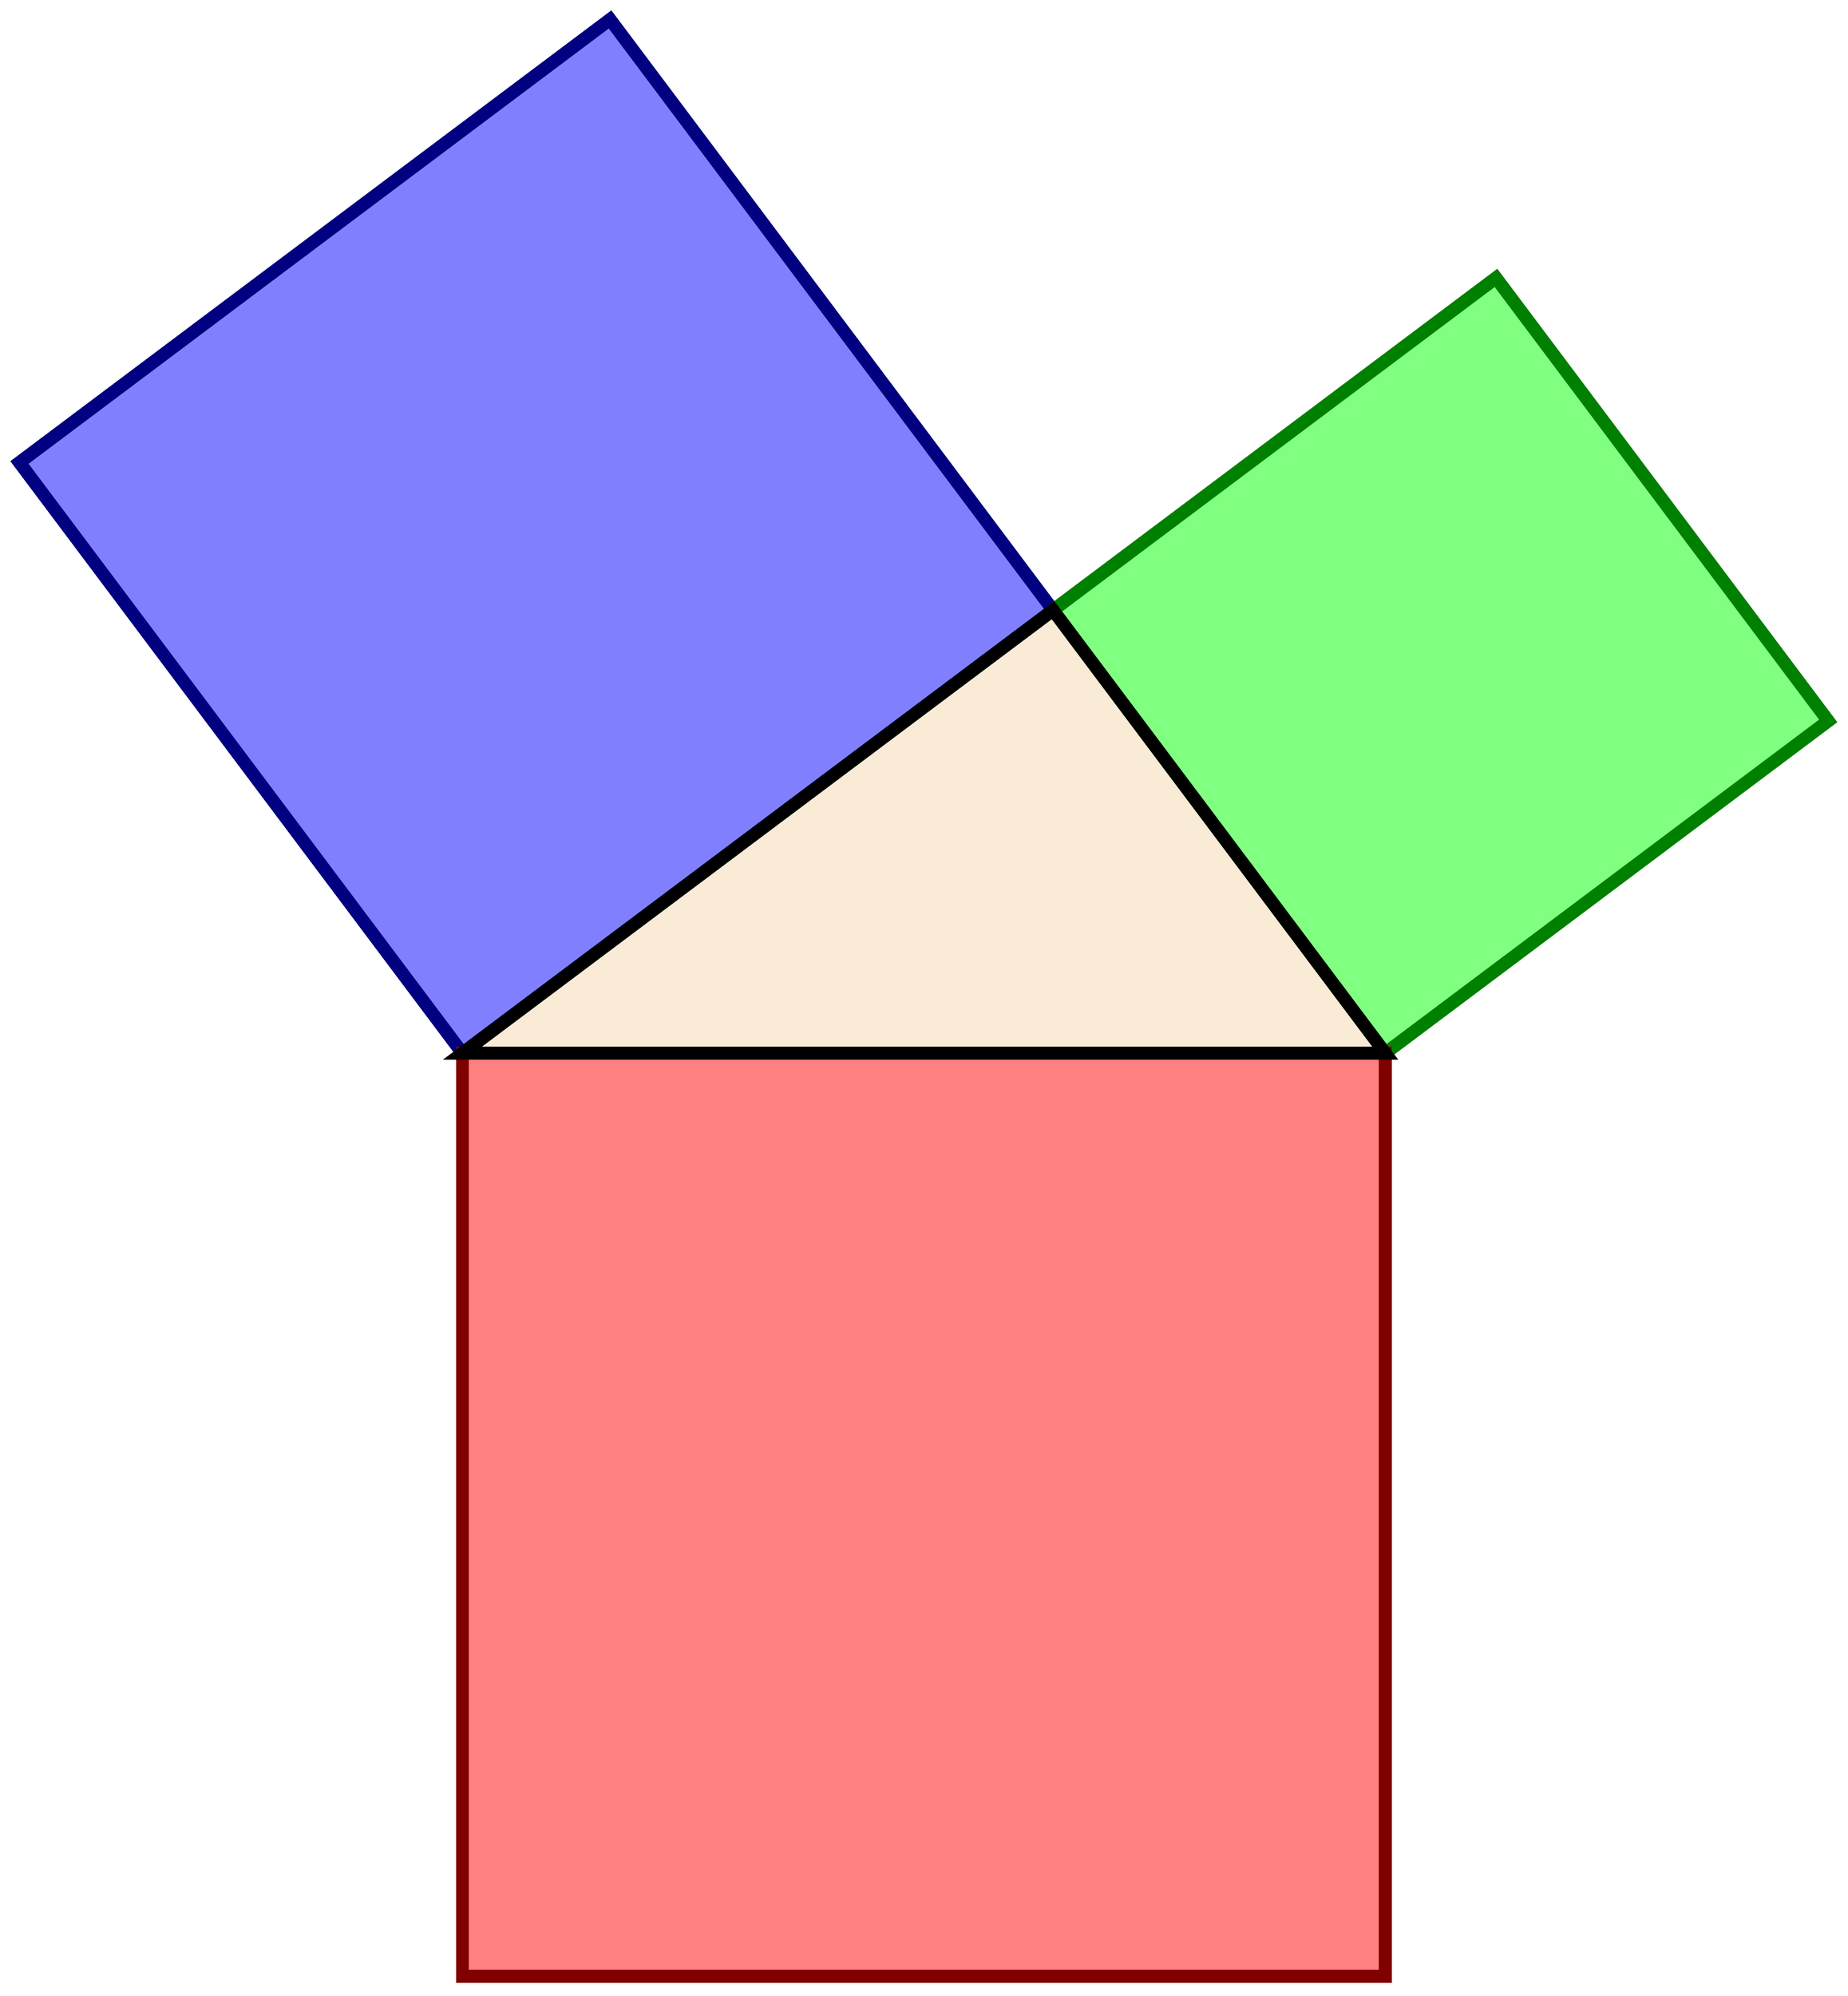
\begin{tikzpicture}[line width=10pt, line cap=round]
  \coordinate (A) at (0,0);
  \coordinate (B) at (16, 12);
  \coordinate (C) at (25, 0);

  \draw[color=blue!50!black, fill=blue!50] (A) -- (B) -- (4, 28) -- (-12, 16) -- cycle;
  \draw[color=green!50!black, fill=green!50] (B) -- (C) -- (37, 9) -- (28, 21) -- cycle;
  \draw[color=red!50!black, fill=red!50] (C) -- (A) -- (0, -25) -- (25, -25) -- cycle;
  \draw[fill=antiquewhite] (A) -- (B) -- (C) -- cycle;
\end{tikzpicture}

\end{document}
